\chapter{روش انجام پروژه}
\section{مقدمه}
برای اجرای این پروژه، روش‌های مختلفی مورد بررسی قرار گرفت تا بتوان بهترین روش را به‌طور موثر  بر روی پهپاد پیاده‌سازی کرد. در نهایت، استفاده از سه شبکه عصبی پیچشی به صورت متوالی به عنوان بهترین راه‌حل انتخاب شد. این سه شبکه به ترتیب وظایف زیر را بر عهده دارند:

\begin{enumerate}
    \item \textbf{آشکارسازی موقعیت کف دست}: هر فریم گرفته‌شده از دوربین پهپاد به ورودی این مدل داده می‌شود. پس از پردازش، خروجی مدل یک جعبه محدودکننده \LTRfootnote{Bounding Box} دست را تولید می‌کند که موقعیت دقیق دست را در تصویر مشخص می‌سازد.
    
    \item \textbf{تشخیص نقاط کلیدی دست}: جعبه مرزی دست که از مدل اول به دست آمده است، به عنوان ورودی به مدل دوم داده می‌شود. این مدل جعبه مرزی را برش زده و ۲۱ نقطه کلیدی سه‌بعدی دست به همراه شاخص دست (راست یا چپ) را تولید می‌کند، که این ویژگی‌ها شامل مفاصل انگشتان و نقاط مهم دست می‌باشند.
    
    \item \textbf{پیش‌بینی علائم دست}: ورودی این مدل، یک ماتریس به ابعاد ۲۱×۲ است که مختصات طول و عرض هر نقطه کلیدی دست را شامل می‌شود. به دلیل محدودیت پهپادها در اندازه‌گیری عمق تصویر و اهمیت کمتر عمق در تشخیص علائم‌های مد نظر، فقط مختصات دوبعدی استفاده می‌شود. خروجی این مدل، پیش‌بینی علائم دست کاربر است. این پروژه ۹ علائم گوناگون را مد نظر قرار داده است (کاربر می‌تواند علائم‌های جدیدی اضافه کند). بنابراین، خروجی شبکه پیچشی شامل ۱۰ کلاس است که ۹ کلاس برای علائم‌های مختلف و یک کلاس برای زمانی که هیچ کدام از علائم‌های موجود تشخیص داده نشود، در نظر گرفته شده است.
\end{enumerate}

این سه مدل با همکاری یکدیگر، از تشخیص  مختصات دست تا پیش‌بینی علائم دست را به صورت بهینه و کارآمد انجام می‌دهند، به‌طوری‌که می‌توانند روی پهپادهای موجود پیاده‌سازی شوند و در کاربردهای واقعی مورد استفاده قرار گیرند. بهینه‌سازی‌ها و پیش‌پردازش‌های انجام‌شده در این پروژه،  این اطمینان را حاصل می‌کنند که سیستم با سرعت و دقت بالا عمل کرده و مناسب برای محیط‌های بی‌درنگ باشد.


\begin{figure}[h]
    \centering
    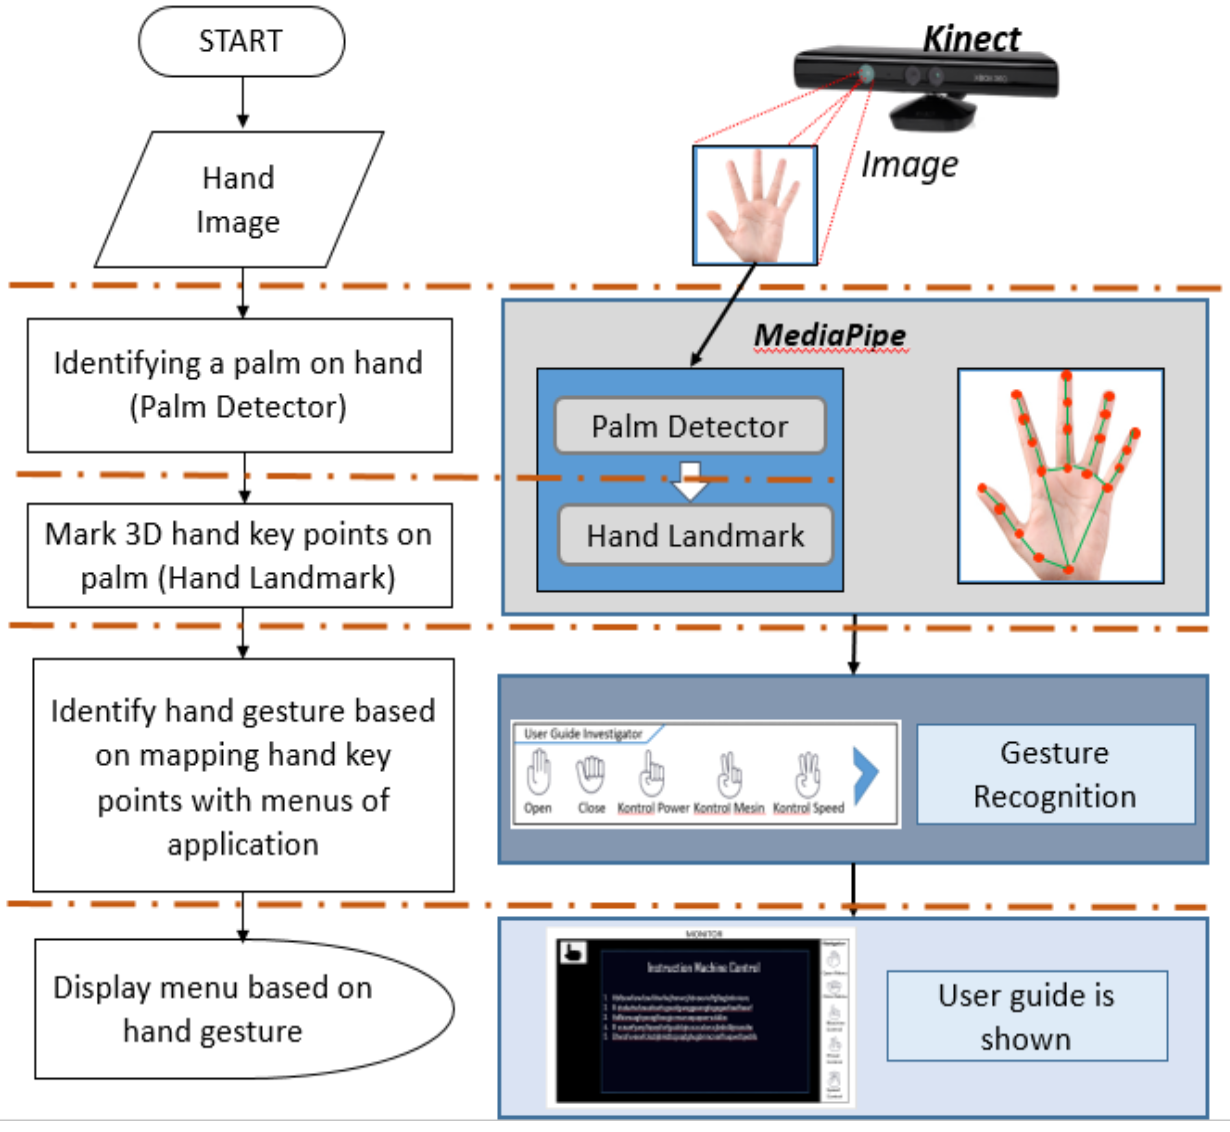
\includegraphics[width=0.8\textwidth]{gesture.png}
    \caption[تشخیص علائم دست با کمک نقاط کلیدی دست]{تشخیص علائم دست با کمک نقاط کلیدی دست \cite{li2012hand}}
\end{figure}

% \section{انتخاب علائم‌های دست متناسب با حرکت پهپاد}
% انتخاب علائم‌های مناسب برای هر یک از حرکات پهپاد از اهمیت ویژه‌ای برخوردار است. چرا که علائم‌هایی که از لحاظ مفهومی به عملکرد پهپاد شبیه هستند راحت‌تر به خاطر سپرده شده و تجربه دلپذیرتری را در کاربر به وجود می‌آورند. 
% ما برای این پروژه 9 علائم دست را در نظر گرفته‌ایم تا بتوان حرکات پایه پهپاد را با آن‌ها انجام داد. این حرکات شامل: حرکت رو به جلو،  حرکت رو به عقب،حرکت به پایین، حرکت به بالا، حرکت به راست، حرکت به چپ، فرود آمدن، 
% ایستادن در موقعیت کنونی و گرفتن عکس است که نمونه علائم دست آن‌ها با توجه به حرکت پهپاد نشان داده شده است.

\section{انتخاب علائم‌های دست متناسب با حرکت پهپاد}
انتخاب علائم‌های مناسب برای هر یک از حرکات پهپاد از اهمیت ویژه‌ای برخوردار است، زیرا علائم‌هایی که از لحاظ مفهومی به عملکرد پهپاد شبیه هستند، راحت‌تر به خاطر سپرده می‌شوند و تجربه کاربری دلپذیرتری را ایجاد می‌کنند. برای این پروژه، نه علائم دست در نظر گرفته شده است تا حرکات پایه پهپاد با استفاده از آن‌ها انجام شود. 
این حرکات شامل: حرکت رو به جلو، حرکت رو به عقب، حرکت به سمت پایین، حرکت به سمت بالا،
حرکت به راست، حرکت به چپ، فرود آمدن پهپاد، چرخش ۳۶۰ درجه به صورت ساعتگرد و گرفتن عکس است.
این علائم‌ها به گونه‌ای انتخاب شده‌اند که با حرکات پهپاد همخوانی داشته باشند و کاربران بتوانند به راحتی آن‌ها را به خاطر بسپارند و از آن‌ها برای کنترل پهپاد استفاده کنند. نمونه‌های علائم دست متناسب با هر حرکت پهپاد، به طور دقیق در عکس \ref{t} ارائه شده‌اند تا کاربران بتوانند به راحتی از آن‌ها استفاده کنند.

\begin{figure}[h]
    \centering
    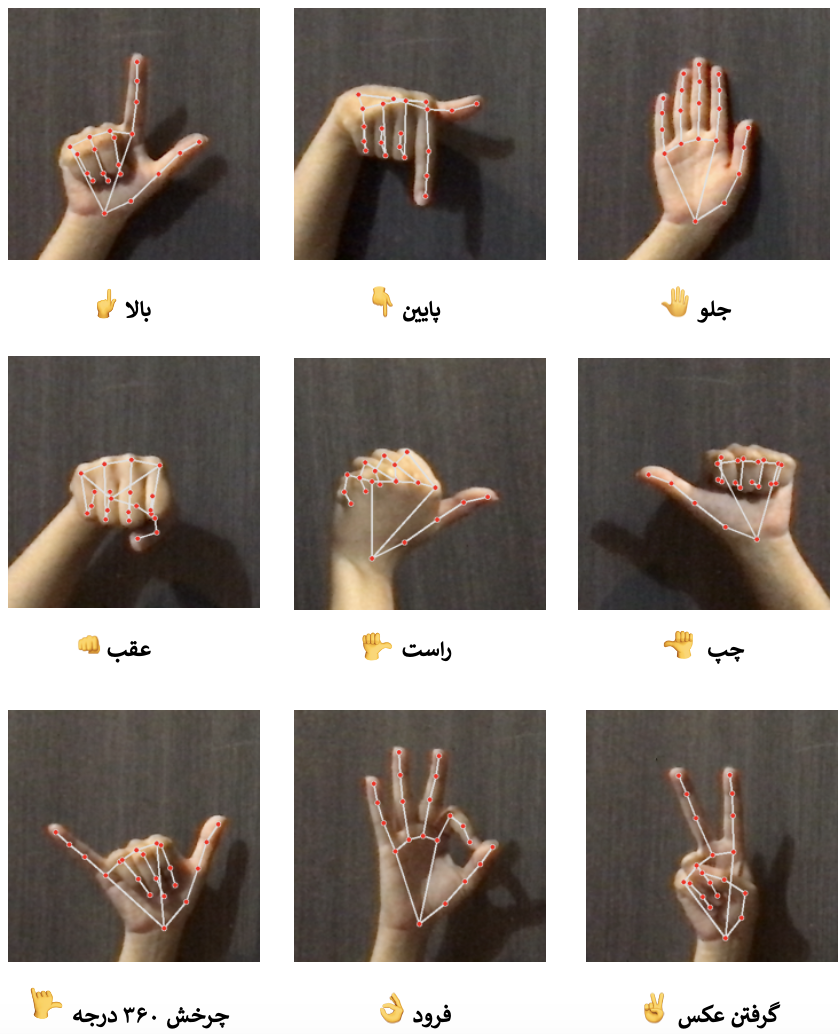
\includegraphics[width=0.7\textwidth]{gestures.png}
    \caption{نمونه‌ای از علائم‌های انتخاب‌شده در مجموعه داده‌ها}
    \label{t}
\end{figure}

\section[مجموع‌داده]{مجموع‌داده \protect\LTRfootnote{Data Set}}
برای جمع‌آوری مجموع‌داده مناسب پروژه، از آنجایی که علائم‌های دست بر اساس عملکرد پهپاد تعیین شدند تا استفاده از آن‌ها برای کاربر مورد پسند باشد، پیدا کردن مجموع‌داده آماده غیرممکن است. جمع‌آوری مجموع‌داده جامع و مناسب از اهمیت
 بالایی برخوردار است زیرا مدل باید به صورت بی‌درنگ کار کند و نمی‌توان از مدل‌های سنگین یادگیری عمیق استفاده کرد. بنابراین، برای افزایش دقت مدل باید از روش‌های دیگری نظیر پیش‌پردازش، پس‌پردازش و استفاده از مجموع‌داده مناسب بهره گرفت.
\\
رویکردهای متفاوتی برای این پروژه پیاده‌سازی شدند تا بهترین راهکار با استفاده از مدلی با حجم کم و در عین حال جامع یافت شود. در نتیجه، مجموع‌داده‌های گوناگونی جمع‌آوری شدند که هر یک از آن‌ها ویژگی خاصی از تصویر
 را به عنوان داده‌ی مورد نیاز جمع‌آوری می‌کردند. این رویکردها شامل استفاده از ورودی کل عکس به صورت پیکسل‌های رنگی، پیدا کردن دست و ذخیره موقعیت آن به صورت پیکسل‌های $256 \times 256$ و پیدا کردن نقاط کلیدی دست و ذخیره موقعیت آن‌ها در مجموع‌داده بود. در نهایت، گزینه سوم به عنوان بهترین راه ممکن برای ذخیره داده‌ها و اجرای پروژه انتخاب شد.

برای این پروژه، به منظور امکان اضافه کردن علائم دست جدید توسط کاربر، کدی پیاده‌سازی شد که با باز شدن دوربین و زدن یک حرف 
یا کلمه یکسان برای هر کلاس، اطلاعات آن تصویر استخراج شده و در مجموع‌داده ذخیره شود. این روش نه تنها جمع‌آوری داده را راحت‌تر می‌کند، بلکه به کاربر اجازه می‌دهد با زدن یک دکمه، کلاس جدیدی را ایجاد کند.


\section{اهمیت علائم دست}
هنگام صحبت کردن، افراد از حرکات دست استفاده می‌کنند. حرکت‌های دست جزء اساسی زبان هستند که اطلاعات معنادار و منحصر به فردی را منتقل می‌کنند. این حرکات به گوینده کمک می‌کنند تا اهداف خود
 را بهتر منعکس کند و نقش‌های مهمی در ارتباط، یادگیری و درک هم برای افرادی که آن‌ها را مشاهده می‌کنند و هم برای کسانی که آن‌ها را انجام می‌دهند ایفا می‌کنند.
\\
به حرکات خود به خودی دست که در ریتم گفتار ایجاد می‌شوند، حرکات هم‌گفتاری \LTRfootnote{Co-Speech Gestures} گفته می‌شود. مردم از تمامی فرهنگ‌ها و پیشینه‌های زبانی شناخته شده برای ارتباط بهتر از حرکات هم‌گفتاری استفاده می‌کنند. حتی نوزادان قبل از بیان اولین کلمات خود، از انواع علائم‌ها استفاده می‌کنند. دست‌ها به ما کمک می‌کنند صحبت کنیم، فکر کنیم و به خاطر بسپاریم، گاهی اوقات دانشی را که هنوز
 نمی‌توان به زبان آورد، آشکار می‌کنند. به طوری که می‌توان گفت علائم‌های دست اغلب به عنوان زبان گفتاری ثانویه در نظر گرفته می‌شوند \cite{clough2020role}.
\\
علائم‌های دست به‌ویژه زمانی مؤثر هستند که مزیتی نسبت به کلمات داشته باشند \cite{kang2016hands}. توانایی درک شکل و حرکت دست‌ها می‌تواند یک
 جزء حیاتی در بهبود تجربه کاربر \LTRfootnote{User Experience} در حوزه‌ها و پلتفرم‌های مختلف فناوری باشد. درک مفهوم علائم دست به صورت بی‌درنگ برای افراد به طور طبیعی وجود دارد، اما این کار زمانی که توسط هوش مصنوعی و بینایی ماشین رخ دهد می‌تواند چالش‌برانگیز باشد. زیرا
دست‌ها اغلب خود یا یکدیگر را مسدود می‌کنند مانند انسداد انگشت، کف دست و حتی لرزش دست نیز می‌تواند مشکلاتی به وجود آورد \cite{zhang2020mediapipe}.


\section{کنترل پهپاد}
اکثر پهپادهای تجاری موجود در بازار یا دارای کنترلرهای ویژه طراحی شده هستند، یا از فرستنده‌های سیگنال اختصاصی و برنامه‌های نرم‌افزاری استفاده می‌کنند که روی
 دستگاه‌های دستی کاربران مانند تلفن‌های همراه یا تبلت‌ها اجرا می‌شوند. در هر دو حالت، کنترل‌کننده فرمان‌هایی را با اطلاعات دقیق از طریق کانال‌های بی‌سیم مانند وای‌فای یا بلوتوث ارسال می‌کند. 
\\
اخیراً محصولات تجاری معرفی شده‌اند که از حرکات دست به عنوان یک مکانیسم کنترل قابل اجرا استفاده می‌کنند. برای دریافت علائم‌ها، دو رویکرد اصلی وجود دارد:
\begin{itemize}
    \item \textbf{استفاده از دستکش‌های ویژه طراحی شده:} کنترل‌کننده بر روی دستکشی که توسط کاربران استفاده می‌شود نصب می‌گردد و در زمان واقعی انحراف، گام و چرخش دست را شناسایی می‌کند تا حرکات مربوط به پهپاد را تشخیص و ارسال کند. از جمله این محصولات می‌توان به \lr{Kd Interactive Aura Drone} و \lr{MenKind Motion Control Drone} اشاره کرد.
    \item \textbf{استفاده از بینایی ماشین از طریق دوربین:}   این دستگاه‌ها از دوربین نصب شده روی پهپاد استفاده می‌کنند تا بتوانند در لحظه تشخیص دهند که دست کاربر کجاست و در چه حالتی قرار دارد تا پهپاد را کنترل کنند. از جمله این محصولات می‌توان به پهپاد دی‌جی‌آی اسپارک \LTRfootnote{DJI Spark Drone} اشاره کرد.
\end{itemize}


\section{ابزار‌ها و نرم افزار های مورد استفاده}
برای پیاده‌سازی این پروژه از ابزار‌ها، نرم‌افزار‌ها و کتاب‌خانه‌های گوناگونی استفاده شده‌است که در ادامه به توضیح دقیق آن‌ها می‌پردازیم. قابل ذکر است که از کتاب‌خانه‌هایی از جمله سی‌اس‌وی \LTRfootnote{Csv}،کپی \LTRfootnote{Copy}، ایترتولز\LTRfootnote{Itertools} و اواس\LTRfootnote{Os} نیز در قسمت‌هایی از پروژه به‌کار برده‌شده است که به دلیل استفاده جزئی توضیح داده نشده‌اند.

% \subsection{زبان برنامه‌نویسی پایتون}

\subsection[کتاب‌خانه تنسورفلو]{کتاب‌خانه تنسورفلو ‌\protect\LTRfootnote{TensorFlow}}
تنسورفلو یک کتاب‌خانه نرم‌افزاری رایگان و منبع باز برای یادگیری ماشین و هوش مصنوعی است. این کتاب‌خانه توسط گوگل برین توسعه داده‌شده و می‌تواند در طیف وسیعی 
از وظایف یادگیری ماشین مورد استفاده قرار گیرد. همچنین تمرکز ویژه‌ای بر آموزش و استنتاج شبکه‌های عصبی عمیق دارد. 
\\
تنسورفلو انعطاف‌پذیری بالایی را دارد که می‌تواند برای انواع مختلف مدل‌های یادگیری ماشین از جمله شبکه‌های عصبی پیچشی، شبکه‌های عصبی بازگشتی و شبکه‌های مولد متخاصم\LTRfootnote{Generative Adversarial Network} مورد استفاده قرار گیرد.
تنسورفلو قابلیت اجرای مدل‌ها بر روی پردازنده‌های چندگانه، پردازنده‌های گرافیکی\LTRfootnote{Graphics Processing Unit} و واحد پردازشی تنسو\LTRfootnote{Tensor Processing Unit} را دارد. همچنین به دلیل محبوبیت و پشتیبانی گسترده،
منابع آموزشی و کتاب‌خانه‌های جانبی فراوانی برای آن وجود دارد. به طور کلی،تنسورفلو یکی از ابزارهای قدرتمند و پرکاربرد در حوزه یادگیری ماشین و هوش مصنوعی است \cite{Introduc60:online}.


\subsection[کتاب‌خانه سایکیت لرن]{کتاب‌خانه سایکیت لرن\protect\LTRfootnote{Scikit-learn}}
سایکیت لرن که با نام‌های \lr{Scikits.learn} و \lr{Sklearn} نیز شناخته می‌شود یک کتاب‌خانه یادگیری ماشین رایگان و منبع باز برای زبان برنامه‌نویسی پایتون است. این کتاب‌خانه شامل الگوریتم‌های مختلفی برای طبقه‌بندی،
رگرسیون و خوشه‌بندی مانند ماشین‌های بردار پشتیبان، جنگل‌های تصادفی
\LTRfootnote{Random Forest}
، تقویت گرادیان
\LTRfootnote{Gradian activation}
،میانگین-کی \LTRfootnote{K-means} و دی‌بی اسکن\LTRfootnote{DBSCAN} می‌باشد. سایکیت لرن به طور ویژه برای تعامل با
کتاب‌خانه‌های  نام‌پای\LTRfootnote{NumPy} و سای‌پای\LTRfootnote{SciPy} طراحی شده است و ابزارهای متنوعی برای پیش‌پردازش داده‌ها، انتخاب و ارزیابی مدل‌ها و کاهش بعد فراهم می‌کند. این کتاب‌خانه به کاربران کمک می‌کند تا به راحتی از آن در پروژه‌های 
یادگیری ماشین استفاده کنند. این کتاب‌خانه به دلیل سادگی و کارایی خود در بین محققان و مهندسان داده بسیار محبوب است و امکانات وسیعی را برای توسعه و ارزیابی مدل‌های یادگیری ماشین فراهم می‌کند \cite{scikitle22:online}.

\subsection[رابط برنامه‌نویسی کراس]{رابط برنامه‌نویسی کراس\protect\LTRfootnote{Keras}}
کراس یک رابط برنامه‌نویسی\LTRfootnote{Application Programming Interface} یادگیری عمیق است که به زبان پایتون نوشته شده و می‌تواند بر روی  تنسورفلو و پای‌تورچ \LTRfootnote{PyTorch} اجرا شود. هدف اصلی کراس کاهش پیچیدگی‌ها و بار شناختی توسعه‌دهندگان است، 
به طوری که آن‌ها بتوانند روی بخش‌های حیاتی و مهم پروژه‌های یادگیری ماشین تمرکز کنند. این رابط برنامه‌نویسی با رابط کاربری ساده و کاربرپسند، امکان توسعه سریع مدل‌های پیچیده را فراهم
می‌کند. کراس عملکرد بالایی دارد و توسط سازمان‌های بزرگی نظیر ناسا، یوتیوب و \lr{Waymo} برای تحلیل داده‌ها، بهبود الگوریتم‌های توصیه‌گر و توسعه سیستم‌های خودران مورد استفاده قرار 
می‌گیرد. این کتاب‌خانه با مستندات جامع و پشتیبانی از جامعه کاربری بزرگ، به یکی از ابزارهای محبوب در حوزه یادگیری عمیق تبدیل شده‌است \cite{AboutKer57:online}.

% \subsection{کتاب‌خانه‌های\lr{MediaPipe}}
% \lr{MediaPipe} مجموعه ای از کتاب‌خانه ها و ابزارهایی است که از تکنیک‌های هوش مصنوعی و یادگیری ماشین در برنامه‌های خود استفاده می‌کند.
% این کتاب‌خانه برای برنامه‌نویسان یادگیری ماشین از جمله محققان، دانشجویان و توسعه‌دهندگان نرم‌افزار، که برنامه‌های کاربردی یادگیری ماشین را پیاده‌سازی می‌کنند، نمونه‌های
% اولیه فناوری را طراحی می‌کند تا بتوان پروژه‌ها را تا حد امکان ساده کرد.
% برنامه‌هایی که داده‌های حسی مثل ویدیو و صدا را با نرخ فریم بالا پردازش می‌کند تا تجربه کاربر را بهتر کند. مراحل پردازش یا مدل‌های استنتاجی ممکن است دشوار باشد، چون 
% گاهی اتصال بین مراحل زیاد است. همچنین، توسعه برنامه برای پلتفرم‌ زمان‌بر است \cite{lugaresi2019mediapipe}. 
% \\
% \lr{Media Pipe} این چالش‌ها را با انتزاع و اتصال مدل‌های مختلف به یکدیگر در یک چارچوب مناسب حل می‌کند. با استفاده از \lr{MediaPipe}، می‌توان یک لوله پردازش را به صورت 
% گراف از اجزای مختلف، از جمله مدل‌های استنتاجی و عملکردهای پردازش رسانه‌ای، ساخت.
% همچنین این کتاب‌خانه می‌تواند مطابق با نیازهای افراد خود سفارشی شود و در پلتفرم‌های مختلف توسعه پیدا کند.
% \\
% در مجموعه \lr{MediaPipe} نیز از کتاب‌خانه‌های مختلفی برای پیاده‌سازی برنامه ها استفاده می‌شود. از جمله آن‌ها می‌توان به \lr{TensorFlow}، \lr{PyTorch}، اپن سی‌وی، \lr{CNTK} و \lr{MXNet} اشاره کرد \cite{harris2021applying}. 


\subsection[کتاب‌خانه‌های مدیاپایپ]{کتاب‌خانه‌های مدیاپایپ \protect\LTRfootnote{MediaPipe}}
مدیاپایپ مجموعه‌ای از کتاب‌خانه‌ها و ابزارهایی است که از تکنیک‌های هوش مصنوعی و یادگیری ماشین در برنامه‌های خود استفاده می‌کند. این کتاب‌خانه برای برنامه‌نویسان یادگیری ماشین از جمله محققان، دانشجویان و توسعه‌دهندگان
 نرم‌افزار، که برنامه‌های کاربردی یادگیری ماشین را پیاده‌سازی می‌کنند، نمونه‌های اولیه و از پیش آموزش دیده‌ای را طراحی می‌کند تا پروژه‌ها را تا حد امکان ساده کند.
\\
برنامه‌هایی که داده‌های حسی مانند ویدیو و صدا را با نرخ فریم بالا پردازش می‌کنند و به‌طور خاص برای بهبود تجربه کاربر
 طراحی شده‌اند چالش‌های محتلفی دارند. برای مثال مراحل پردازش یا مدل‌های استنتاجی ممکن است پیچیده باشند، زیرا گاهی اتصال بین مراحل بسیار زیاد است. همچنین، توسعه برنامه برای پلتفرم‌های مختلف نیز می‌تواند زمان‌بر باشد \cite{lugaresi2019mediapipe}. 
\\
مدیاپایپ این چالش‌ها را با انتزاع و اتصال مدل‌های مختلف به یکدیگر در یک چارچوب مناسب حل می‌کند. با استفاده از مدیاپایپ، می‌توان یک لوله پردازش را به صورت گراف از اجزای مختلف، از جمله مدل‌های استنتاجی و عملکردهای پردازش رسانه‌ای، ساخت. این کتاب‌خانه همچنین قابل سفارشی‌سازی است و می‌تواند بر روی پلتفرم‌های مختلف توسعه یابد.
\\
در مجموعه مدیاپایپ نیز از کتاب‌خانه‌های مختلفی برای پیاده‌سازی برنامه‌ها استفاده می‌شود. از جمله آن‌ها می‌توان به تنسورفلو، پای‌تورچ، اپن سی‌پی
\LTRfootnote{OpenCv}
، \lr{CNTK} و \lr{MXNet} اشاره کرد \cite{harris2021applying}.


\begin{figure}[h]
    \centering
    \includegraphics[width=0.85\textwidth]{mediapipe2.png}
    \caption[برخی کاربردهای کتاب‌خانه مدیاپایپ]{برخی کاربردهای کتاب‌خانه مدیاپایپ \cite{harris2021applying}}
\end{figure}

\subsection{کتاب‌خانه نام‌پای}
نام‌پای کتاب‌خانه‌ای برای محاسبات علمی در پایتون است که آرایه‌های چندبعدی و توابعی برای عملیات سریع  بر روی این آرایه‌ها ارائه می‌دهد. در هسته‌ی نام‌پای، شیء \lr{Ndarray} وجود 
دارد که آرایه‌های \lr{n}-بعدی تشکیل شده از داده‌های همگن را در بر می‌گیرد و بسیاری از عملیات‌های ریاضی بر روی آن‌ها انجام می‌شود. این کتاب‌خانه امکان انجام عملیات ریاضی پیشرفته و سایر 
عملیات‌ها روی تعداد زیادی داده را با کارایی بالا فراهم می‌کند، که نسبت به استفاده از توابع از پیش تعریف شده زبان برنامه‌نویسی پایتون کارآمدی و حجم کد کمتری دارد \cite{WhatisNu62:online}.

\subsection[کتاب‌خانه مت‌پلات لیب]{کتاب‌خانه مت‌پلات لیپ \LTRfootnote{Matplotlib}}
مت‌پلات لیپ یک کتاب‌خانه چند پلتفرمی\LTRfootnote{Cross-Platform}، برای تجسم داده‌ها و نمودارهای گرافیکی از جمله هیستوگرام، نمودارهای پراکنده و نمودار میله‌ای برای زبان برنامه‌نویسی
پایتون است. توسعه دهندگان همچنین می توانند از رابط‌های برنامه‌نویسی مت‌پلات لیپ برای جاسازی نمودارها در برنامه‌های دارای رابط کاربری گرافیکی نیز استفاده کنند.
\\
یک آغازگر
\LTRfootnote{Script}
مت‌پلات لیپ  درون زبان برنامه‌نویسی پایتون به گونه‌ای ساختار یافته است که چند خط کد تنها چیزی است که در بیشتر موارد برای تولید نمودار داده بصری مورد نیاز است. مت‌پلات لیپ دو رابط برنامه‌نویسی را پوشش می دهد:
\\
رابط برنامه‌نویسی پای‌پلات \LTRfootnote{Pyplot}، که سلسله مراتبی از اشیاء درون کد پایتون است که در بالای آن \lr{Matplotlib.Pyplot} قرار دارد. و رابط برنامه‌نویسی اشیاء گرا\LTRfootnote{Object Oriented} که می تواند 
با انعطاف پذیری بیشتری نسبت به \lr{Pyplot} سرهم شوند. این رابط برنامه‌نویسی دسترسی مستقیم به لایه‌های پشتی مت‌پلات لیب
\LTRfootnote{Matplotlib Backend}
را فراهم می کند \cite{Introduc75:online}.

\subsection{کتاب‌خانه اپن سی‌وی}
اپن سی‌وی یک کتاب‌خانه متن باز برای بینایی ماشین و یادگیری ماشین است که برای فراهم کردن زیرساخت مشترک برای برنامه‌های بینایی ماشین و تسریع استفاده از ادراک ماشین در محصولات
تجاری طراحی شده است. این کتاب‌خانه شامل بیش از 2500 الگوریتم بهینه‌سازی شده است که مجموعه جامعی از الگوریتم‌های کلاسیک و جدید بینایی ماشین و یادگیری ماشین 
را فراهم می‌کند. اپن سی‌وی به طور گسترده‌ای در شرکت‌ها، گروه‌های تحقیقاتی و نهادهای دولتی برای انجام پروژه‌های بینایی ماشین و یادگیری ماشین استفاده می‌شود. این کتاب‌خانه رابط‌های برنامه‌نویسی 
متعددی از جمله 
سی پلاس پلاس، پایتون ،جاوا و متلب را دارد که امکان انجام پروژه‌های بینایی ماشین با استفاده از زبان‌های برنامه‌نویسی مختلف را فراهم می‌کند \cite{AboutOpe4:online}.

\subsection{پهپاد دی‌جی‌آی تلو}
پهپاد دی‌جی‌آی تلو یک پهپاد کوادکوپتر کوچک و قابل برنامه‌ریزی است که برای مصارف آموزشی و تست پروتوتایپ توسط شرکت دی‌جی‌آی طراحی شده است. این پهپاد دارای ویژگی‌های ویژه‌ای مانند حرکات پایه‌ای کوادکوپتری و همچنین تکنولوژی 
کنترل پرواز دی‌جی‌آی و یک پردازنده بسیار قوی از شرکت اینتل است. دوربین 5 مگاپیکسلی این پهپاد امکان ضبط ویدیو با کیفیت مناسب را فراهم می‌کند. همچنین، پهپاد دارای یک سیستم موقعیت‌یابی بصری\LTRfootnote{Vision Positioning System} است که شامل 
یک دوربین و یک ماژول مادون قرمز 3 بعدی است و قادر است در فواصل سه تا سی متر ارتفاع  را کار کند .
\\
هسته پهپاد به عنوان مرکز پردازشی و کنترلی آن عمل می‌کند و از یک پردازنده اینتل قدرتمند پشتیبانی می‌کند. پهپاد دی‌جی‌آی تلو برای اجرای پروژه‌های هوش مصنوعی مانند تشخیص اشیاء روی پهپاد، از زبان 
برنامه‌نویسی پایتون و بسته توسعه نرم‌افزار مربوطه پشتیبانی می‌کند. این بسته توسعه نرم‌افزار به کاربران این امکان را می‌دهد که نمونه‌های اولیه پروژه‌های خود را توسعه دهند و آن‌ها را بر روی پهپاد اجرا کنند .
\\
این پهپاد دارای یک باتری با ویژگی‌های خاصی مانند زمان پرواز زیاد و زمان شارژ کم است که می‌تواند از نظر عملکرد و ماندگاری باتری نسبت به پهپاد‌های دیگر مزیت داشته باشد. همچنین، پروژه‌های هوش مصنوعی که روی پهپاد دی‌جی‌آی تلو پیاده‌سازی می‌شوند، 
می‌توانند شامل تشخیص اشیاء، پیش‌بینی حرکت‌ها و یا حتی خودکارسازی فرآیندهای پروازی باشند. از جمله مدل‌های هوش مصنوعی که می‌تواند روی پهپاد دی‌جی‌آی تلو پیاده‌سازی شود، می‌توان به یولو سه \LTRfootnote{YOLOv3} اشاره کرد که برای تشخیص اشیاء با دقت بالا استفاده می‌شود \cite{bhujbal2022custom}.

\begin{figure}[h]
    \centering
    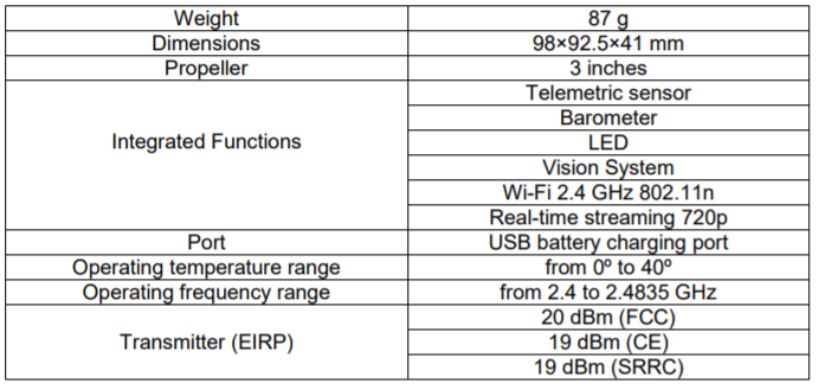
\includegraphics[width=0.8\textwidth]{table.png}
    \caption[طلاعات پهپاد دی‌جی‌آی تلو]{اطلاعات پهپاد دی‌جی‌آی تلو \cite{bhujbal2022custom}}
\end{figure}


\section[روندنمای اجرای پروژه]{روندنمای \protect\LTRfootnote{Flow Chart} اجرای پروژه}
در این پروژه از ۳ مدل اصلی به صورت متوالی برای پیش‌بینی تعیین علائم دست استفاده شده‌ است. این سه مدل شامل تشخیص مرز‌های دست، تشخیص نقاط کلیدی دست و در نهایت تعیین علائم دست است. پس از استفاده از این مدل‌های بینایی ماشین، دستور پیش‌بینی شده برای اجرا به پهپاد دی‌جی‌آی تلو فرستاده می‌شود.
\\
برای بهینه کردن روند این پروژه ماژول‌های گوناگونی از جمله محدود كننده جريان بی‌درنگ، تشخيص با استفاده از مستطيل محدودکننده، برش تصوير،  ورود نقاط عطف به مستطيل محدودکننده و ارائه كننده حاشيه نويسي نیز پیاده‌سازی شده‌اند تا روند پیش‌بینی علائم دست را با سرعت و دقت بالاتری اجرا کنند.

\begin{figure}[h]
    \centering
    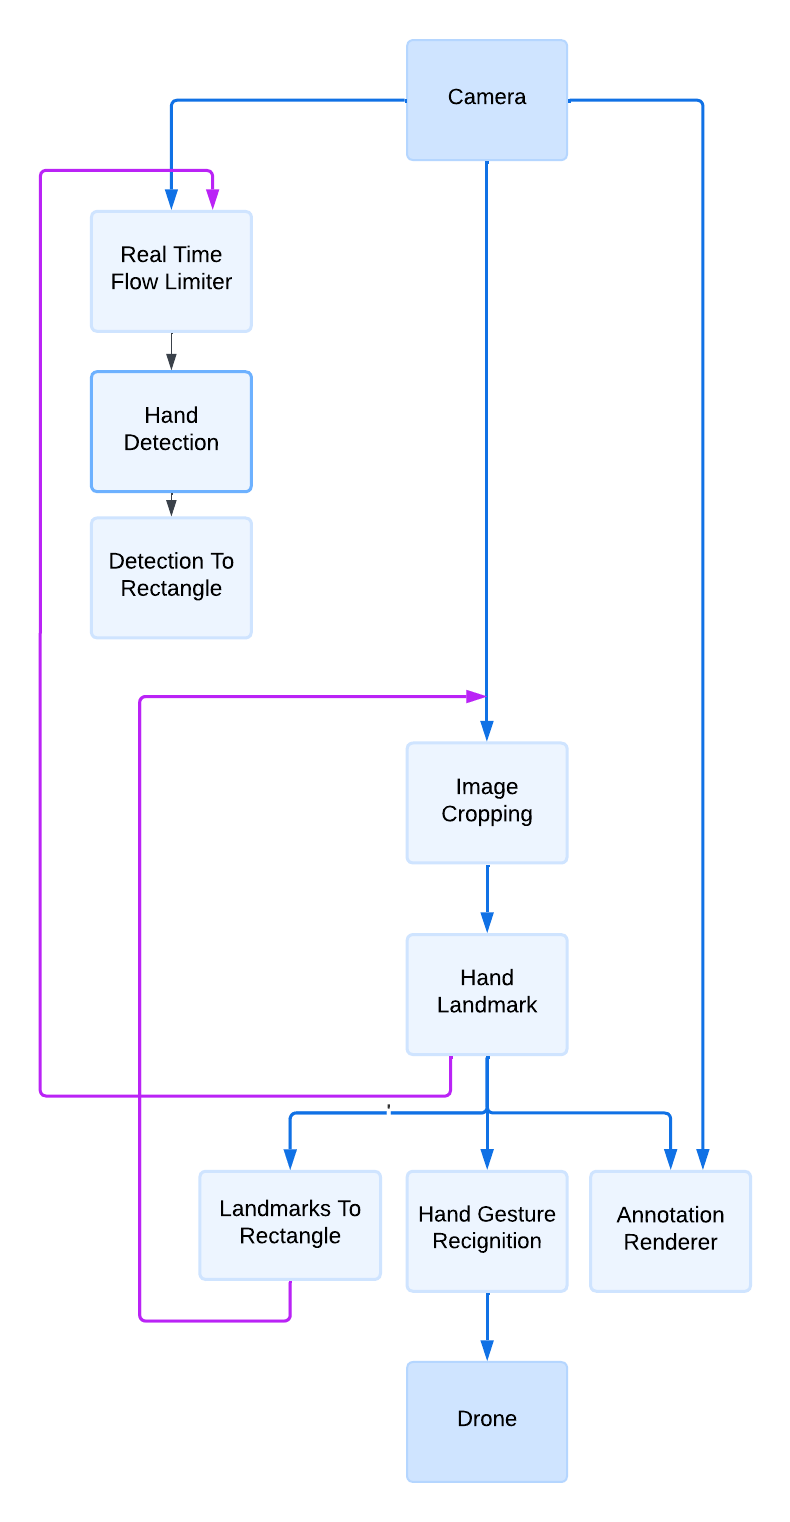
\includegraphics[width=0.5\textwidth]{flowchart.png}
    \caption{فلوچارت پروژه}
\end{figure}



% \section{مدیاپایپ}
% برای پیاده سازی شبکه‌های تشخیص کف دست و پیدا کردن نقاط عطف دست از مدل‌های از قبل آموزش دیده\LTRfootnote{Pretrained} کتاب‌خانه مدیاپایپ کمک گرفته‌شده است. مدیاپایپ  از یک خط لوله
% یادگیری ماشین متشکل از چندین مدل که با هم کار می‌کنند استفاده می‌کند: یک مدل تشخیص کف دست \LTRfootnote{Palm Detection Model}
% که تصویر را از ورودی می‌گیرد و  عکس محدوده دست را به عنوان خروجی دریافت می‌کند و یک مدل تشخیص نقاط عطف دست \LTRfootnote{Hand Landmark Model}
% که عکس دست را به عنوان ورودی گرفته و مختصات‌ 21 نقطه کلیدی بند‌های انگشتان دست را در ناحیه دست تشخیص می‌دهد.
% در عکس \ref{Chart} ماژول‌های مربوط به شناسایی نقاط کلیدی نشان داده‌شده که به تفکیک هر کدام را توضیح خواهیم داد.

% \begin{figure}[h]
%     \centering
%     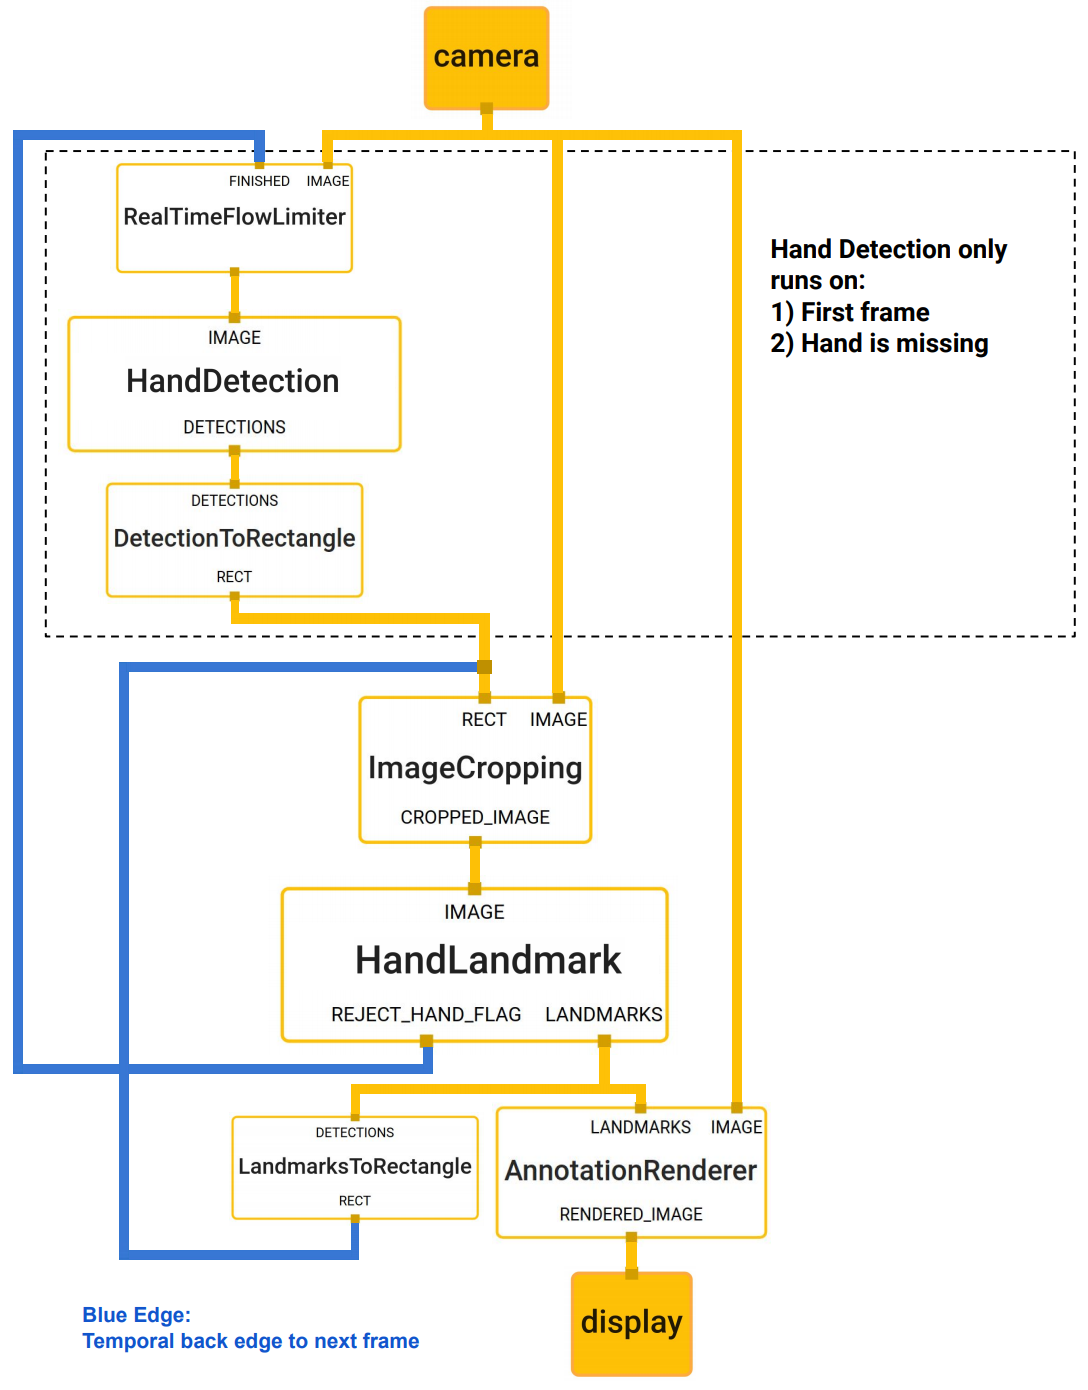
\includegraphics[width=0.7\textwidth]{hand_chart.png}
%     \caption{نمودار \lr{MediaPipe} برای شناسایی نقاط کلیدی دست}
%     \label{chart}
% \end{figure}



\subsection[تشخیص دست]{تشخیص دست\protect\LTRfootnote{Hand Detection}}
ماژول تشخیص دست، یکی از سه ماژول اصلی است که با دقت متوسط ۷.۹۵ درصد عمل می‌کند. این دقت بالا با استفاده از استراتژی‌های مختلف به دست آمده است. این ماژول به جای تشخیص دست، 
از یک مدل تشخیص کف دست استفاده می‌کند زیرا تشخیص محدوده‌های اجسام سفت و سخت مانند کف دست و مشت بسیار ساده‌تر از تشخیص دست‌ها با انگشتان مفصلی است. در این ماژول از
 الگوریتم سرکوب غیر حداکثری برای حذف تشخیص‌های تکراری و انتخاب مرتبط‌ترین اشیاء شناسایی شده استفاده می‌شود که به کاهش نتیجه‌های مثبت کاذب و پیچیدگی محاسباتی کمک می‌کند و وظیفه اصلی آن تشخیص دست در تصویر و محاسبه مکان دقیق دست است.

این ماژول قادر است به‌صورت دقیق و کارآمد موقعیت دست‌ها را شناسایی کند و نواحی مربوطه را برای
 پردازش‌های بعدی فراهم کند. ورودی این ماژول شامل تصویر یا فریم ویدیو است، در حالی که خروجی آن شامل مستطیل‌های محدوده دست‌ها، نمرات اطمینان و در صورت فعال بودن، دست غالب\LTRfootnote{Handedness} است. معماری این ماژول شامل 
 مراحل پیش پردازش\LTRfootnote{Preprocessing}،مدل تشخیص دست و پس پردازش\LTRfootnote{Postprocessing} است که به ترتیب شامل نرمال‌سازی و تغییر اندازه تصویر، شبکه عصبی تشخیص دست و فیلترینگ و محاسبه نواحی مستطیلی دست‌ها می‌باشد.

وظیفه اصلی ماژول شناسایی و محصور کردن دست‌ها در تصاویر و ویدیوها است که در کاربردهای مختلفی از جمله تشخیص حرکات دست، رابط‌های کاربری بدون لمس، تحلیل رفتار و علائم‌ها و کمک به افراد کم‌توان
 اهمیت دارد. این ماژول به توسعه‌دهندگان این امکان را می‌دهد که به راحتی و با دقت بالا دست‌ها را در تصاویر و ویدیوها شناسایی کرده و از این اطلاعات برای پردازش‌های بعدی استفاده کنند.


\begin{figure}[h]
    \centering
    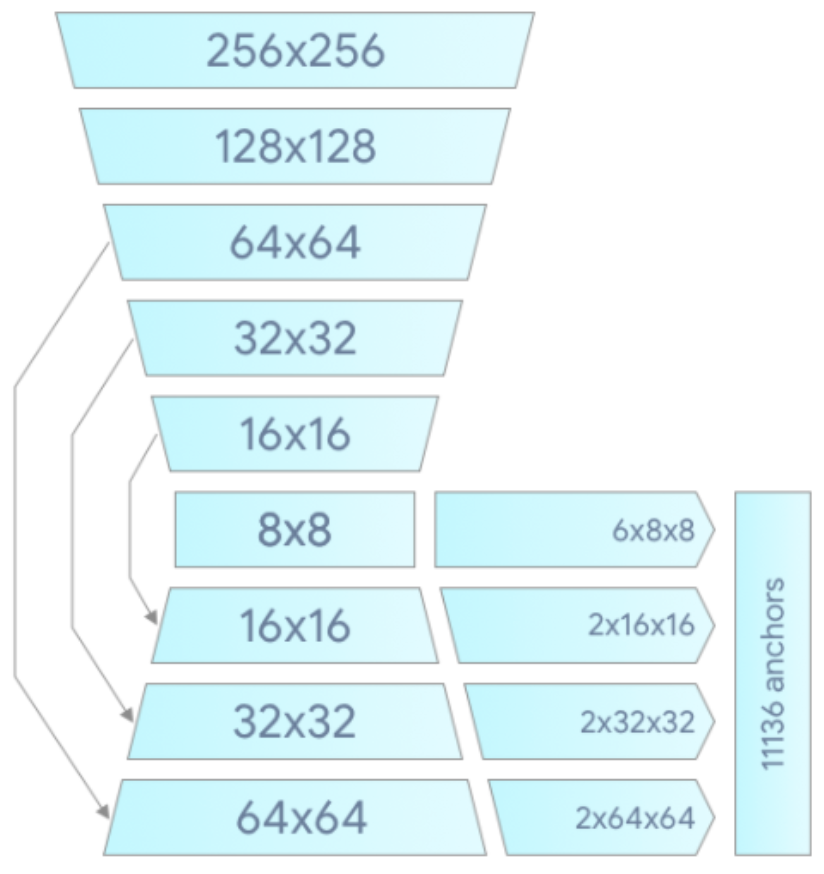
\includegraphics[width=0.4\textwidth]{hand_detector.png}
    \caption[معماری مدل آشکارساز کف دست]{معماری مدل آشکارساز کف دست\cite{zhang2020mediapipe}}
\end{figure}


\subsection{تشخیص نقاط عطف دست\protect\LTRfootnote{Hand Landmark}}
این ماژول یکی دیگر از ماژول‌های مدل اصلی است که یک ابزار قدرتمند برای تشخیص و ردیابی نقاط کلیدی دست است. این ماژول وظیفه تشخیص و محاسبه نقاط عطف دست را بر عهده دارد. ورودی آن یک تصویر است که شامل دست یا دست‌هایی 
است که می‌خواهیم نقاط کلیدی آن‌ها را تشخیص دهیم. این تصویر باید از پیش‌پردازش شده و دارای جعبه‌ی مرزی‌ای باشد که دست در آن قرار دارد که توسط ماژول تشخیص دست مشخص شده است.
\\
خروجی این ماژول شامل موقعیت سه‌بعدی بیست و یک نقطه کلیدی دست است که شامل مفاصل انگشتان و نوک انگشتان می‌باشد. این نقاط کلیدی به صورت مجموعه‌ای از مختصات طول, عرض و ارتفاع ارائه می‌شود 
که طول و عرض نشان دهنده موقعیت هر نقطه را در فضای دوبعدی و ارتفاع نشان‌دهنده عمق نقطه نسبت به تصویر ورودی است.
\\
معماری این ماژول شامل  شبکه‌های عصبی عمیق است که از آن‌ها برای تشخیص و ردیابی نقاط کلیدی دست استفاده می‌کند. این معماری شامل مراحل پیش‌پردازش برای تغییر اندازه و نرمال‌سازی تصویر، تشخیص دست برای شناسایی ناحیه‌های دست، مدل 
نقاط عطف برای تشخیص دقیق نقاط کلیدی دست و پس‌ پردازش برای تبدیل مختصات نقاط کلیدی به فرمت خروجی نهایی و اعمال اصلاحات لازم است.
\\
وظیفه اصلی این ماژول تشخیص و ردیابی دقیق نقاط کلیدی دست‌ها در تصاویر و ویدیوها است. این قابلیت می‌تواند در برنامه‌های مختلفی مانند واقعیت افزوده \LTRfootnote{Augmented Reality}، رابط‌های کاربری بدون لمس،
تحلیل حرکات، تشخیص حرکات دست در زبان اشاره و ... استفاده شود و توسعه‌دهندگان را قادر می‌سازد از این قابلیت‌های پیشرفته در برنامه‌های خود بهره ببرند \cite{zhang2020mediapipe}.

\begin{figure}[h]
    \centering
    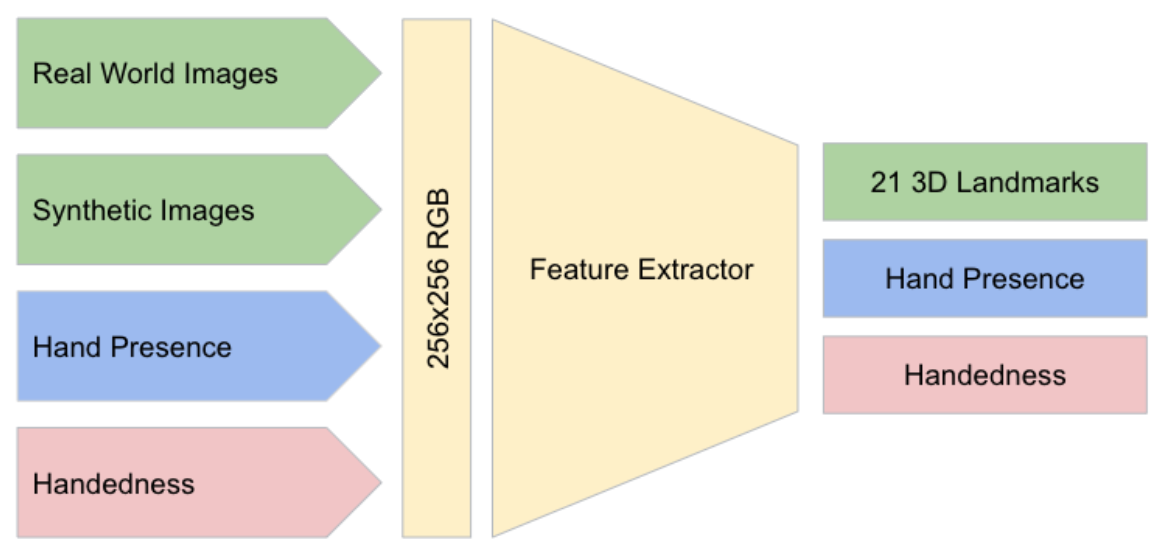
\includegraphics[width=0.7\textwidth]{landmark.png}
    \caption[معماری مدل نقطه عطف دست]{معماری مدل نقطه عطف دست. این مدل دارای سه خروجی است که یک استخراج کننده ویژگی را به اشتراک می‌گذارند. هر سر توسط مجموعه داده های مربوطه که با همان رنگ مشخص شده اند آموزش داده می‌شود \cite{zhang2020mediapipe}.}
\end{figure}

\begin{figure}[h]
    \centering
    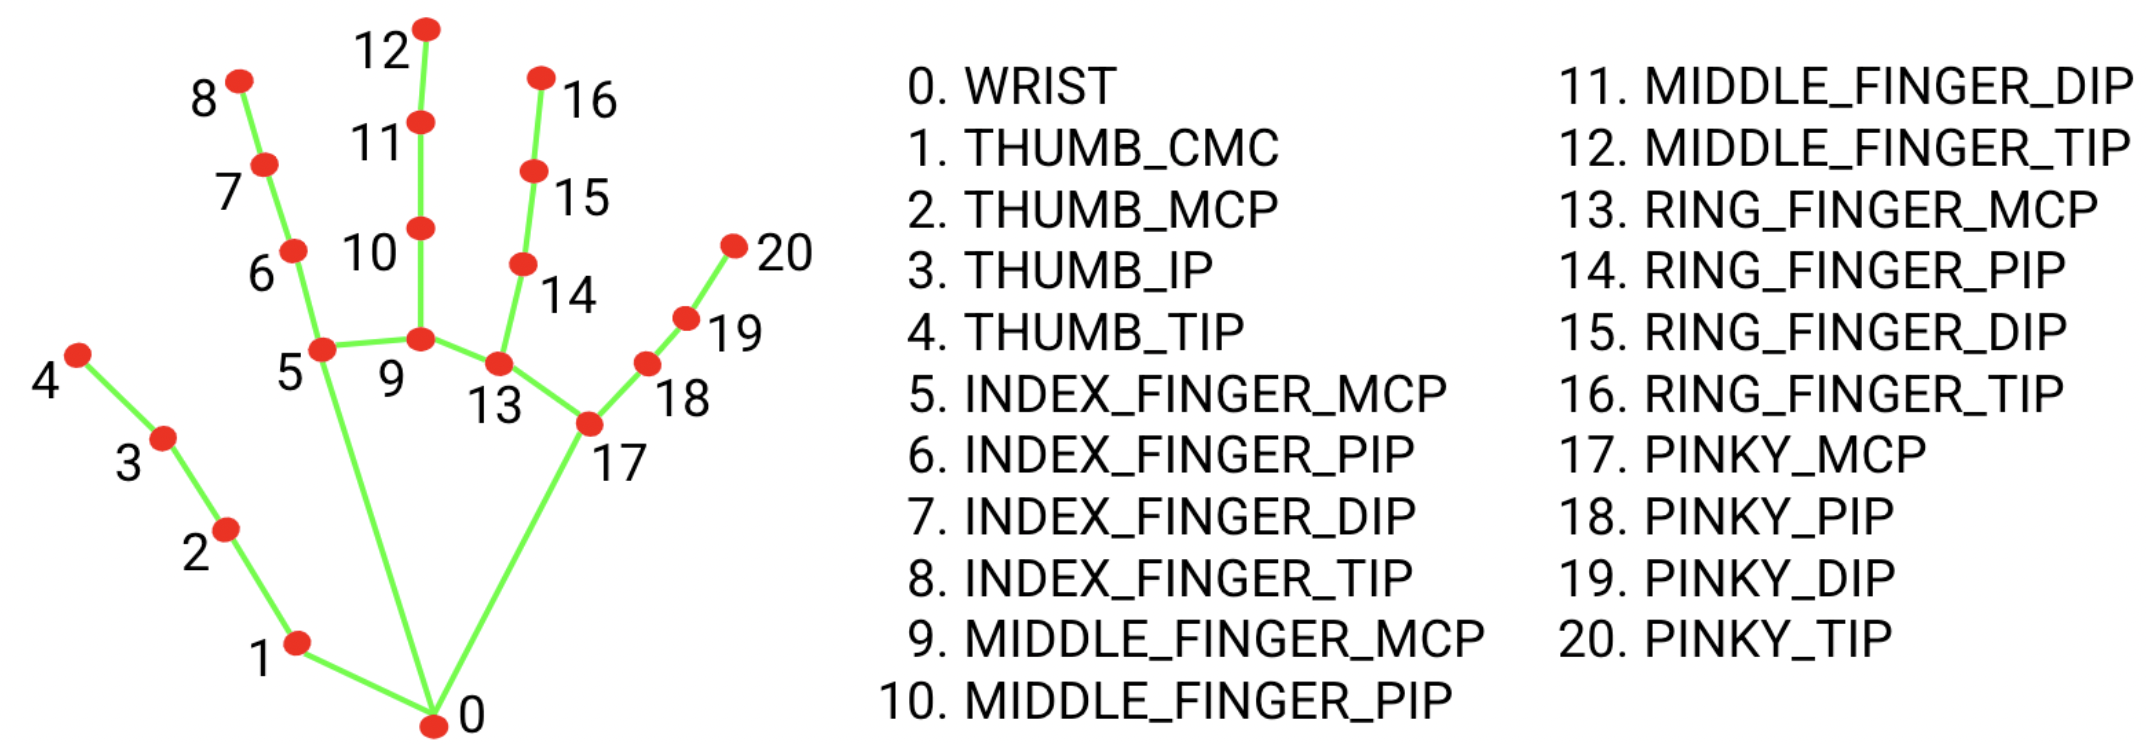
\includegraphics[width=1\textwidth]{hand-landmarks.png}
    \caption[موقعیت ۲۱ نقطه کلیدی در ناحیه دست]{موقعیت ۲۱ نقطه کلیدی در ناحیه دست \cite{zhang2020mediapipe}}
\end{figure}


\subsection{پیش‌بینی علائم دست}
برای پیش‌بینی علائم دست از مدل‌های گوناگونی استفاده شده است که معماری و مشخصات هر یک در ادامه به تفکیک توضیح داده‌ شده‌اند. این معماری‌ها شامل شبكه چندلایه‌ای پرسپترونی، شبكه عصبي پیچشی، شبكه عصبي بازگشتي و شبكه‌هاي حافظه كوتاه مدت بلند مدت است. دلیل استفاده از این مدل‌ها حجم کم و در عین حال دقت بالای آن‌ها است تا بتوان آن‌ها را با یکدیگر قیاس و در نهایت بهترین مدل را برگزید. 
ورودی این مدل نقاط کلیدی دست و خروجی آن پس از پردازش شامل ۱۰ کلاس است. شایان ذکر است که کاربر توانایی اضافه کردن کلاس و در نتیجه علائم جدید را نیز در صورتی که پهپاد قابلیت انجام آن را داشته باشد دارد.

\begin{figure}[h]
    \centering
    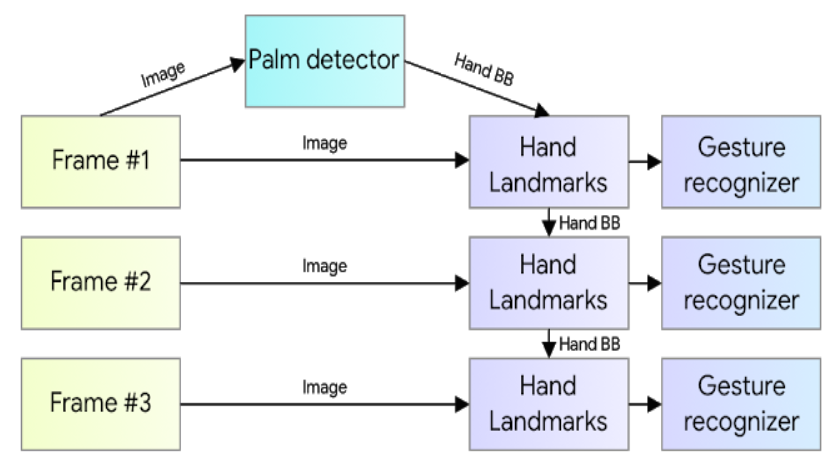
\includegraphics[width=0.7\textwidth]{mediapipe.png}
    \caption[خط لوله تشخیص علائم دست]{خط لوله تشخیص علائم دست \cite{zhang2020mediapipe}}
\end{figure}

\subsection{محدود کننده جریان بی‌درنگ\protect\LTRfootnote{Real Time Flow Limiter}}
ماژول محدود کننده جریان بی‌درنگ وظیفه محدود کردن جریان پردازش به سرعت بی‌درنگ را بر عهده دارد. این ماژول امکان کنترل پردازش داده‌ها را به صورت کارآمد و بی‌درنگ بدون ایجاد تأخیر یا بار اضافی 
بر سیستم فراهم می‌کند.  ورودی‌های این ماژول شامل جریان‌های بسته\LTRfootnote{Packet Streams} و مهر زمان‌ها \LTRfootnote{Time Stamp} و خروجی‌های آن شامل جریان‌های بسته با نرخ محدود\LTRfootnote{Rate-Limited Packet Streams} و اطلاعات مربوط به 
بسته‌های حذف شده ناشی از محدودیت نرخ پردازش است. معماری این ماژول شامل مراحل بافر ورودی\LTRfootnote{Input Buffering} ،تجزیه و تحلیل مهر زمانی\LTRfootnote{Timestamp Analysis} ،الگوریتم محدود کردن نرخ\LTRfootnote{Rate Limiting Algorithm}  و
بافر خروجی\LTRfootnote{Output Buffering} است که به منظور محدود کردن نرخ جریان داده‌ها و انجام پردازش به صورت بی‌درنگ طراحی شده است. این ماژول کمک می‌کند تا بار پردازش و تأخیر کاهش یابد، کیفیت خدمات حفظ شود و منابع محاسباتی بهینه‌سازی شوند \cite{zhang2020mediapipe}.


\subsection{تشخیص به مستطیل محدودکننده\protect\LTRfootnote{Detection To Rectangle}}
این ماژول وظیفه تبدیل نتایج تشخیص اشیاء به مستطیل‌های محدودکننده دست را دارد. این ماژول ورودی‌هایی مانند تشخیص پروتوی\LTRfootnote{Detection Proto} و فریم تصویر\LTRfootnote{Image Frame} را دریافت کرده و مستطیل‌های محدودکننده را به صورت 
نرمال‌سازی شده و یا مطلق برای نواحی تشخیص داده شده تولید می‌کند. معماری این ماژول شامل مراحل  پیش‌پردازش، تبدیل تشخیص\LTRfootnote{Detection Conversion} و پس‌پردازش است. وظیفه اصلی آن تبدیل نتایج تشخیص به 
مستطیل‌های محدودکننده است که در کاربردهای مختلف مانند تشخیص و ردیابی چهره، تشخیص دست، امنیتی و واقعیت افزوده کاربرد دارد \cite{zhang2020mediapipe}.

% \begin{figure}[h]
%     \centering
%     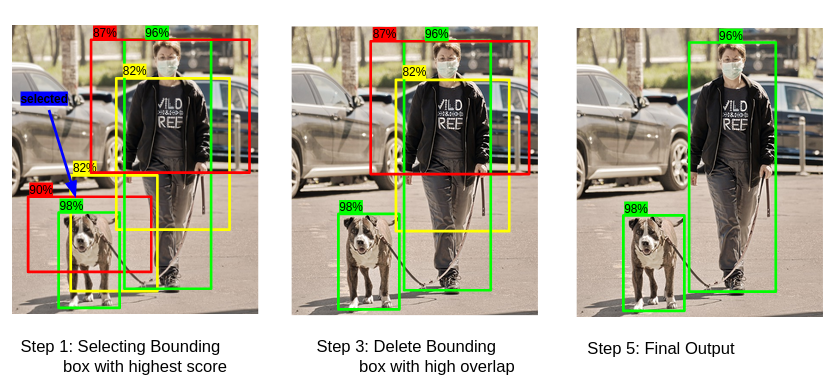
\includegraphics[width=0.55\textwidth]{bounding_box.png}
%     \caption{پیدا کردن مستطیل حاوی دست}
% \end{figure}

\subsection{برش تصویر \protect\LTRfootnote{Image Cropping}}
ماژول برش تصویر برای برش و استخراج ناحیه‌های مورد نظر از تصاویر استفاده می‌شود. این ماژول ورودی‌هایی مانند تصویر اصلی و جعبه مرزی\LTRfootnote{Bounding Box} یا مختصات برش را می‌پذیرد و تصویر برش‌خورده حاوی ناحیه مورد 
نظر را تولید می‌کند. معماری این ماژول شامل مراحل پیش‌پردازش، عملیات برش\LTRfootnote{Cropping Operation}  و پس‌ پردازش  می‌باشد. وظیفه اصلی این ماژول برش دقیق ناحیه‌های مورد نظر از تصویر اصلی است که در کاربردهای 
مختلفی مانند پیش‌پردازش برای تشخیص چهره یا دست، تحلیل تصاویر پزشکی، واقعیت افزوده و پردازش تصویر در کاربردهای امنیتی مورد استفاده قرار می‌گیرد. این ماژول به 
توسعه‌دهندگان این امکان را می‌دهد که ناحیه‌های خاصی از تصاویر را به‌صورت دقیق و مؤثر استخراج کرده و برای پردازش‌های بعدی آماده کنند \cite{zhang2020mediapipe}.


\subsection{نقاط عطف یه مستطیل\protect\LTRfootnote{Landmarks To Rectangle}}
این ماژول برای تبدیل نقاط کلیدی به مستطیل‌های محدودکننده استفاده می‌شود. هدف آن محصور دقیق نقاط کلیدی دست است. با استفاده از این مستطیل‌ها، می‌توان موقعیت دقیق‌تر اشیاء در 
تصویر را نمایش داد و از آن‌ها به عنوان ورودی برای ماژول‌های بعدی در گراف استفاده کرد. این ماژول شامل مراحل پیش‌پردازش داده‌های ورودی، محاسبه مستطیل محدودکننده، نرمال‌سازی مختصات مستطیل‌ها و تولید خروجی نهایی 
 می‌باشد. وظیفه اصلی این ماژول تبدیل نقاط کلیدی به مستطیل‌های محدودکننده دقیق است که در بسیاری از کاربردها اهمیت دارد، از جمله آن‌ها ردیابی اشیاء، تحلیل حرکات، پیش‌پردازش برای مدل‌های دیگر و افزایش دقت در پردازش تصویر است \cite{zhang2020mediapipe}.
تفاوت این ماژول با ماژول اول این است که در ماژول اول ما ورودی خام از تصاویر و یا فریم‌های ویدیو را به عنوان ورودی داده و محدوده دست را تعیین ‌می‌کنیم, اما در 
این ماژول نقاط کلیدی استخراج شده به ماژول داده می‌شوند تا مجدد یک مستطیل محدودکننده برای نقاط عطف استخراح شده تولید کند.

\subsection{ارائه کننده حاشیه نویسی\protect\LTRfootnote{Annotation Renderer}}
این ماژول برای نمایش گرافیکی نتایج پردازش‌های مختلف بر روی تصاویر یا ویدیوها استفاده می‌شود. این ماژول اطلاعات حاشیه‌نویسی شامل نقاط کلیدی، مستطیل‌های محدودکننده، خطوط، متن و سایر اشکال گرافیکی را به صورت 
بصری بر روی تصاویر نمایش می‌دهد. وظیفه اصلی آن شامل نمایش بصری نقاط کلیدی، مستطیل‌های محدودکننده، خطوط و اتصالات، متن و توضیحات بر روی تصاویر یا ویدیوها است. این ماژول به توسعه‌دهندگان امکان 
می‌دهد تا به راحتی و به صورت بصری نتایج پردازش‌های خود را مشاهده کنند و از این طریق به بهبود و ارزیابی عملکرد مدل‌ها و الگوریتم‌های خود بپردازند.
همچنین وجود این ماژول توضیح پذیری مدل‌های یادگیری عمیق استفاده شده را نیز افزایش می دهد
\cite{zhang2020mediapipe}.
% \subsection{مزیت‌های استفاده از کتاب‌خانه \lr{MediaPipe}}

\subsection{مدل‌های استفاده شده در ماژول کلاس‌بندی برای تعیین علائم دست}

\subsection{شبکه عصبی  چندلایه‌ای پرسپترونی}
شبکه عصبی  چندلایه‌ای پرسپترونی \LTRfootnote{Multilayer Perceptron Neural Network} نوعی شبکه عصبی  هوش مصنوعی است که از چندین لایه نورون تشکیل شده است. نورون‌های درون لایه‌ها معمولاً از
توابع فعال‌سازی غیرخطی \LTRfootnote{Nonlinear Activation Functions} استفاده می‌کنند که به شبکه اجازه می‌دهد الگوهای پیچیده در داده‌ها را بیاموزد. شبکه‌های عصبی چندلایه‌ای پرسپترونی در 
یادگیری ماشین اهمیت بالایی دارند زیرا می‌توانند روابط غیرخطی در داده‌ها را یاد بگیرند و آن‌ها را به مدل‌های قدرتمندی برای استفاده در کارهایی مانند طبقه‌بندی، رگرسیون و تشخیص الگو تبدیل کند. 
\\
شبکه عصبی چندلایه‌ای پرسپترونی نوعی شبکه عصبی پیش‌خور\LTRfootnote{Feedforward} است که از نورون‌های کاملاً متصل با یک تابع فعال‌سازی از نوع غیر خطی تشکیل شده است و  برای تشخیص داده‌هایی که به صورت خطی قابل تفکیک نیستند استفاده می‌شود.
\\
شبکه‌های عصبی چندلایه‌ای پرسپترونی به طور گسترده در زمینه‌های مختلف از جمله تشخیص تصویر، پردازش زبان طبیعی و تشخیص گفتار و ... استفاده می‌شوند. انعطاف پذیری آن‌ها در
معماری و توانایی تقریب هر عملکرد تحت شرایط خاص آن‌ها را به یک بلوک اساسی در یادگیری عمیق و تحقیقات شبکه عصبی تبدیل می‌کند. 

\begin{figure}[h]
    \centering
    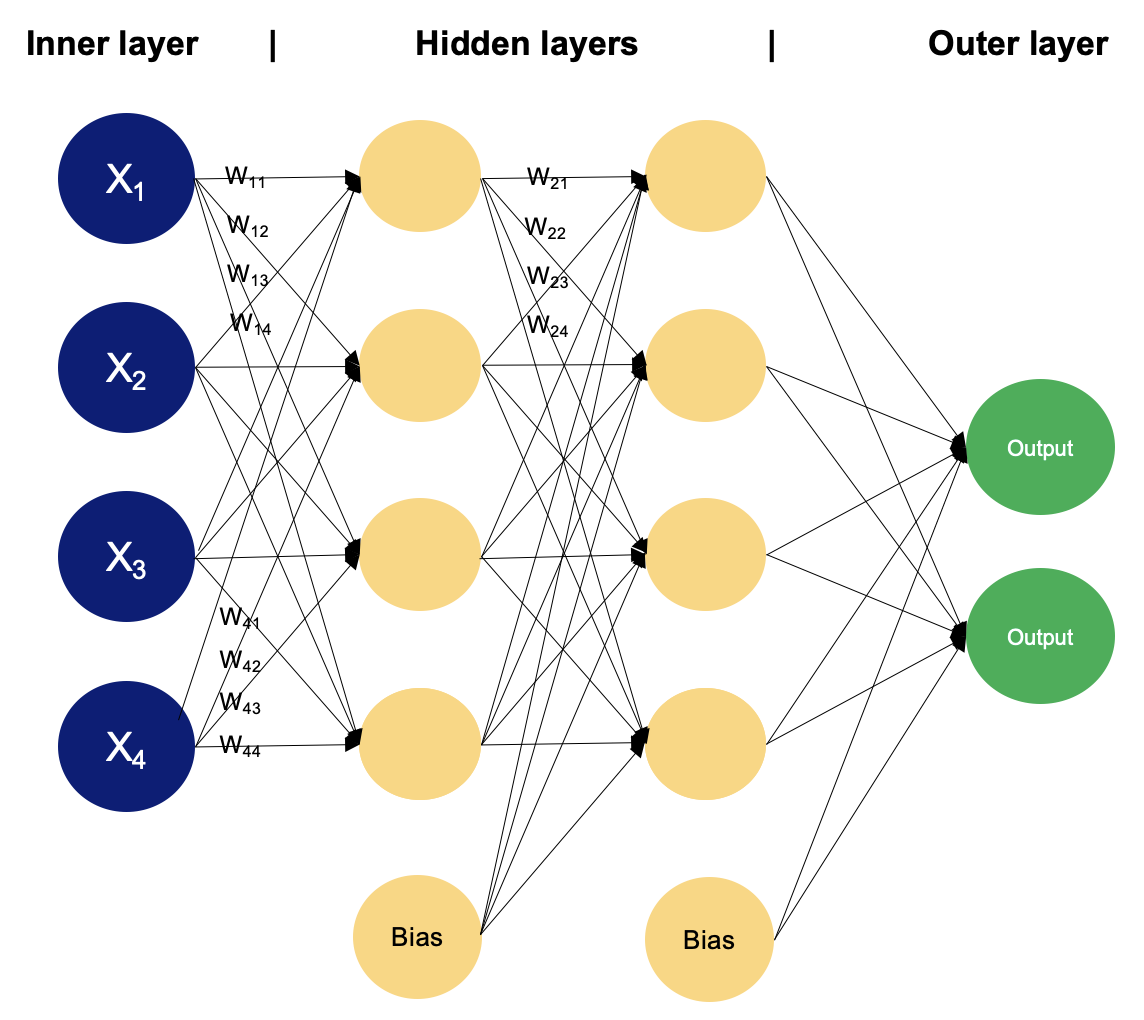
\includegraphics[width=0.6\textwidth]{MLP.png}
    \caption[نمونه ای از شبکه‌های عصبی چند لایه‌ای دارای دو لایه پنهان]{نمونه ای از شبکه‌های عصبی چند لایه‌ای دارای دو لایه پنهان\cite{Multilay58:online}}
\end{figure}


\subsection{شبکه‌ عصبی پیچشی}
شبکه‌های عصبی پیچشی\LTRfootnote{Convolutional Neural Network} یک الگوریتم یادگیری عمیق است که از جمله کاربرد‌های آن در زمینه تشخیص اشیا می‌توان به مواردی مانند طبقه بندی، تشخیص و تقسیم بندی تصویر 
اشاره کرد. بسیاری از برنامه‌های کاربردی مانند اتومبیل های خودران، دوربین های نظارتی و موارد دیگر از شبکه‌های عصبی پیچشی استفاده می‌کنند.
\\
برخلاف مدل‌های سنتی یادگیری ماشین مانند ماشین بردار پشتیبانی و درخت‌ تصمیم
\LTRfootnote{Decision Tree}
که نیاز به استخراج دستی ویژگی‌ها دارند، شبکه‌های عصبی پیچشی می‌توانند استخراج خودکار ویژگی‌ها را در مقیاس‌های بزرگ 
انجام دهند. این ویژگی یکی از دلایل اصلی کارآمد بودن این شبکه‌ها است. این شبکه‌ها می‌توانند الگوهای مختلف را از درون داده‌ها تشخیص دهند و ویژگی‌های داده را بدون توجه به موقعیت آن‌ها، اعم از چرخش، تبدیل‌‌های هندسی و یا جابجایی تصاویر استخراج کنند.
\\
معماری شبکه‌های عصبی پیچشی سعی می‌کنند تا ساختار نورون‌ها را در سیستم بینایی انسان متشکل از چندین لایه تقلید کند، جایی که هر یک مسئول تشخیص یک ویژگی خاص در داده‌ها است. 
همانطور که در 
\cref{cnn_arch}
نیز نشان داده شده است، شبکه عصبی پیچشی از چندین لایه مانند لایه ورودی، لایه پیچشی، لایه ادغام \LTRfootnote{Pooling} و لایه‌های کاملاً متصل تشکیل شده است.
\\
لایه پیچشی فیلترهایی را روی تصویر ورودی اعمال می‌کند تا ویژگی‌ها را استخراج کند, لایه ادغام ابعاد تصویر را کاهش می‌دهد تا محاسبات را سریع‌تر و کمتر کند و لایه کاملاً متصل پیش بینی نهایی را انجام می‌دهد. بدین صورت که شبکه فیلترهای بهینه را از طریق پس انتشار
\LTRfootnote{Back Propagation}
و نزول گرادیان
\LTRfootnote{Gradian Descent}
می‌آموزد.


\begin{figure}[h]
    \centering
    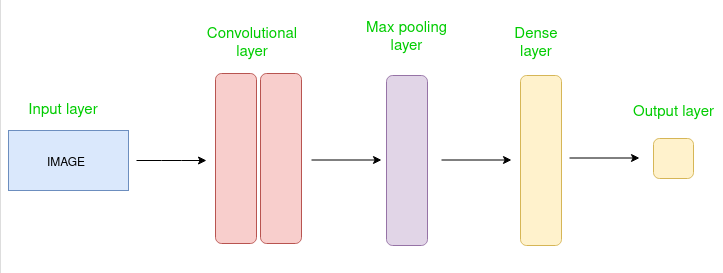
\includegraphics[width=0.9\textwidth]{CNN_arch.png}
    \caption[نمونه معماری شبکه عصبی پیچشی]{نمونه معماری شبکه عصبی پیچشی \cite{Introduc84:online}}\label{cnn_arch}
\end{figure}

\subsection{شبکه عصبی بازگشتی}
شبکه عصبی بازگشتی\LTRfootnote{Recurrent Neural Network}  نوعی شبکه عصبی است که در آن خروجی مرحله قبل به عنوان ورودی به مرحله فعلی داده می‌شود. در شبکه‌های عصبی سنتی، تمامی ورودی‌ها و خروجی‌ها مستقل از یکدیگر 
هستند. برای مثال در مواردی که پیش‌بینی مدل متکی به موارد قبلی است و نیاز است آن‌ها را نیز مدنظر قرار دهد این شبکه بسیار کارآمد است. شبکه عصبی بازگشتی با کمک یک لایه پنهان این امکان را فراهم می‌کند. اصلی‌ترین و مهم‌ترین 
ویژگی شبکه عصبی بازگشتی حالت پنهان آن است که برخی از اطلاعات یک دنباله را به خاطر می‌سپارد. این حالت به عنوان حالت حافظه نیز شناخته می‌شود زیرا ورودی قبلی شبکه را به خاطر می‌آورد. و از پارامترهای یکسانی برای هر 
ورودی استفاده می‌کند زیرا وظیفه یکسانی را روی تمام ورودی‌ها یا لایه‌های پنهان برای تولید خروجی انجام می‌دهد. این بر خلاف سایر شبکه‌های عصبی، پیچیدگی پارامترها را کاهش می‌دهد.


\begin{figure}[h]
    \centering
    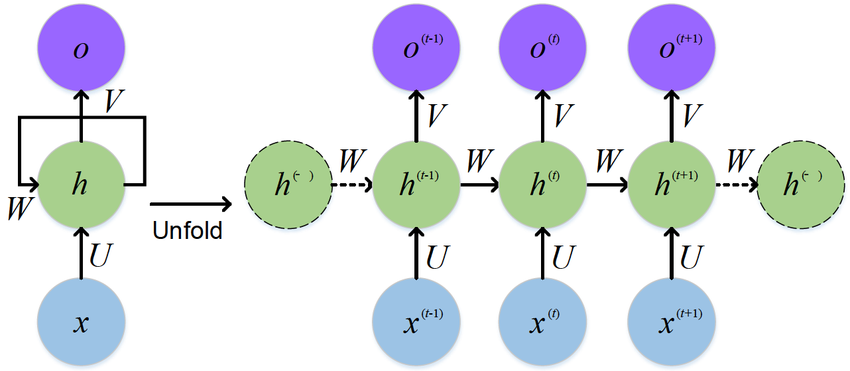
\includegraphics[width=0.8\textwidth]{RNN.png}
    \caption[نمونه معماری شبکه عصبی بازگشتی]{نمونه معماری شبکه عصبی بازگشتی\cite{inproceedings}}
\end{figure}

\subsection{شبکه‌ حافظه طولانی کوتاه مدت}
شبکه عصبی بازگشتی یک حالت پنهان دارد که در طول زمان منتقل می‌شود، این مساله می‌تواند یادگیری وابستگی‌های طولانی مدت را برای شبکه دشوار کند. شبکه‌های حافظه طولانی کوتاه مدت
\LTRfootnote{Long Short-Term Memory }
این مشکل را با معرفی یک سلول حافظه، که این سلول محفظه‌ای است که می‌تواند اطلاعات را برای مدت طولانی نگهداری کند، برطرف می‌کند. شبکه‌های حافظه طولانی کوتاه مدت 
 قادر به یادگیری وابستگی‌های طولانی‌مدت در داده‌های متوالی هستند، که آن‌ها را برای کارهایی مانند ترجمه زبان، تشخیص گفتار و پیش‌بینی 
سری‌های زمانی مناسب می‌سازد. شبکه‌های حافظه طولانی کوتاه مدت همچنین می توانند در ترکیب با دیگر معماری‌های شبکه عصبی، مانند شبکه‌های عصبی پیچشی برای تجزیه و تحلیل تصویر و ویدئو استفاده شوند.
\\
سلول حافظه توسط سه گیت کنترل می‌شود: گیت ورودی، دروازه فراموشی و گیت خروجی. این گیت‌ها تصمیم می‌گیرند که چه اطلاعاتی را به سلول حافظه اضافه، حذف  و از آن خروجی بگیرند. گیت ورودی کنترل می‌کند که چه اطلاعاتی 
به سلول حافظه اضافه می‌شود. دروازه فراموشی کنترل می‌کند که چه اطلاعاتی از سلول حافظه حذف می‌شود. و گیت خروجی کنترل می‌کند که چه اطلاعاتی از سلول حافظه خارج می‌‌شود.
این  گیت به شبکه‌های حافظه طولانی کوتاه مدت اجازه می‌دهد تا به‌طور انتخابی اطلاعات در جریان در شبکه را حفظ  و یا کنار بگذارند، که این ویژگی امکان آموزش وابستگی‌های طولانی‌مدت را برای شبکه فراهم می‌کند .

\begin{figure}[h]
    \centering
    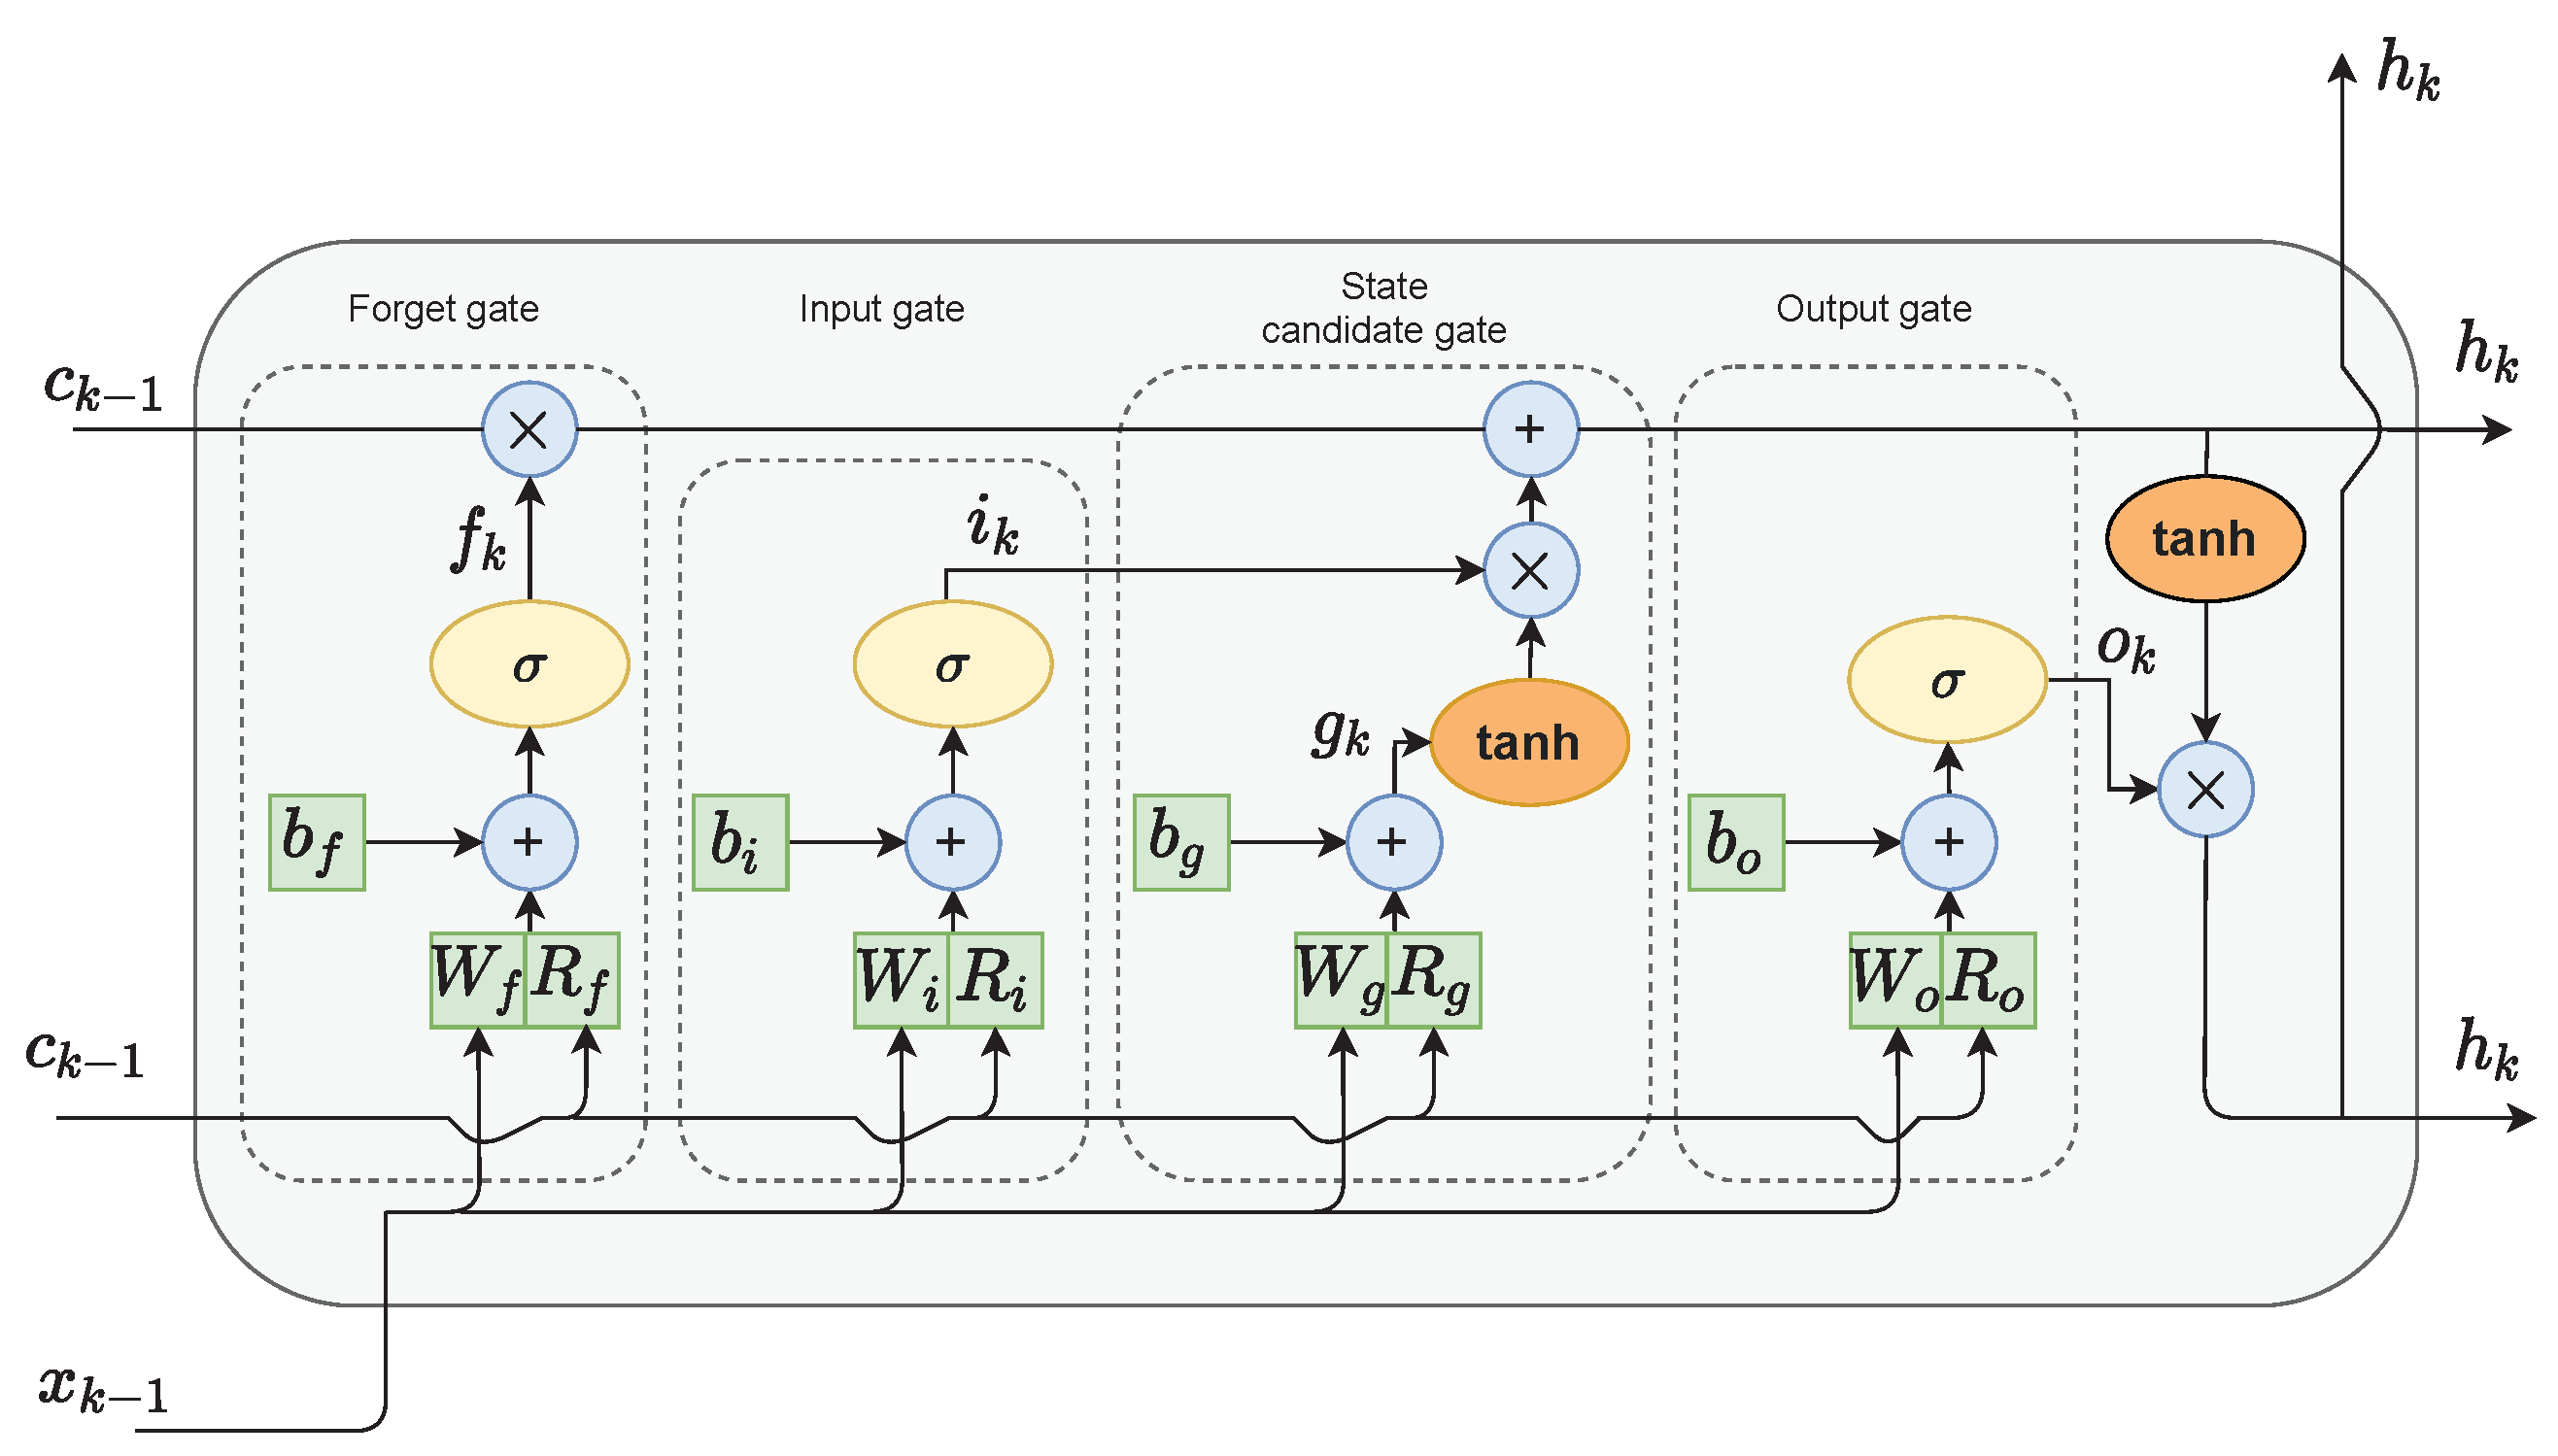
\includegraphics[height=9cm,width=0.9\textwidth]{LSTM.png}
    \caption[نمونه معماری شبکه‌ حافظه طولانی کوتاه مدت]{نمونه معماری شبکه‌ حافظه طولانی کوتاه مدت \cite{s21165625}}
\end{figure}




\section{پیش‌پردازش مدل تشخیص علائم دست}
برای ورود نقاط عطف دست به مدل تعیین علائم به ۲۱ مختصات طول و عرض نیاز داریم. خروجی مدل تعیین مختصات نقاط عطف دست برابر مختصات مطلق پیکسل‌ها نسبت به گوشه سمت 
چپ پایین تصویر است. این نقاط با توجه به اندازه عکس می‌توانند گسترده باشند برای مثال در یک عکس با اندازه ۲۰۴۸*۲۰۴۸ این اعداد از بین ۰ تا ۲۰۴۸ متغیر اند. 
اگر این مختصات را به صورت مستقیم به مدل تعیین علائم دست بدهیم دقت مدل برابر ۸۷ درصد خواهد بود که به میزان کافی مورد قبول نیست. برای بهبود آن باید پیش‌پردازش‌هایی بر روی داده ورودی انجام شود. 
\\
از جمله این پیش‌پردازش‌ها می‌توان به نسبی کردن و نرمال‌سازی داده‌ها اشاره کرد. برای این کار ابتدا باید یک مرجع واحد در نظر گرفت تا نقاط، نسبت به آن مشخص شوند. در این پروژه ما مرجع را نقطه 
مشخص شده روی مچ در نظر می‌گیریم. مختصات نقطه مرجع را برابر (0,0)  قرار می‌دهیم. سپس نسبت به آن و با توجه به
\cref{eq:ref}
مختصات نقاط دیگر را به روز رسانی می‌کنیم.

\begin{equation}\label{eq:ref}
    X_{rel} = X_ref -X
\end{equation}


پس از نسبی کردن نقاط نسبت به مبدأ، آن‌ها را با کمک 
\cref{eq:normal_ref}
نرمال سازی می‌کنیم تا تمام طول و عرض نقاط به عددی میان صفر و یک به روز رسانی شوند.
\begin{equation}\label{eq:normal_ref}
    X_{new} = \frac{X - X_{min}}{X_{max} - X_{min}}
\end{equation}

در انتها این این مختصات را به عنوان ورودی به شبکه تعیین علائم دست می‌دهیم. با توجه به اینکه معماری هیچ یک از مدل‌ها تغییر نکرده است و تنها داده‌های مختصات به روز رسانی شده‌اند، 
دقت نهایی مدل به ۹۷ درصد افزایش پیدا کرده است و پیش‌پردازش تاثیر به‌سزایی در افزایش دقت پروژه داشته است.


% \section{رأی‌گیری پنجره‌ای}
\section{پس‌پردازش مدل تشخیص علائم دست}
با وجود اینکه دقت مدل پیاده‌سازی شده بالا و مقدار قابل قبولی است و عملکرد بسیار چشم‌گیری از خود نشان می‌دهد، در عین حال پیش‌بینی اشتباه مدل می‌تواند عواقب زیان‌باری را به ارمغان آورد، 
از تجربه ناپسند برای کاربر گرفته تا برخورد پهپاد به اجسام و هزینه‌های مالی گزاف. لذا باید دقت انجام پروژه را از آنچه مدل پیش‌بینی می‌کند نیز بالاتر برد. برای این کار از رأی‌گیری پنجره‌ای 
استفاده کرده‌ایم. بدین صورت که متغیری را با توجه به تعداد فریم بر ثانیه دوربین در نظر می‌گیریم. بدین صورت که هر چه تعداد فریم ضبط شده بر ثانیه در دوربین پهپاد بیشتر باشد متغیر در نظر گرفته‌شده نیز بیشتر 
است. در این پروژه از آنجایی که نرخ فریم بر ثانیه دوربین پهپاد برابر با سی است.  مقدار این متغیر را برابر با ده در نظر گرفته شده است.  سپس یک حد بالا بین صفر تا یک برای تایید خروجی نهایی تعریف می‌کنیم. نقدار این متغییر نیز در این پروژه برابر با 7.0 در نظر گرفته شده است . طبق این راه ما ده فریم متناوب گرفته‌شده از پهپاد را به مدل پیاده‌سازی شده می‌دهیم اما تنها در صورتی دستور پیش‌بینی شده را به 
پهپاد می‌دهیم که حد ممکن را بدست آورند. برای مثال اگر هفت یا بیشتر از ده حرکت پیش بینی شده، دستور حرکت رو به جلو باشد آنگاه به پهپاد دستور داده می‌شود تا به جلو حرکت کند. 
در غیر این صورت اگر کمتر از هفت عدد از فریم‌ها یک   حرکت یکسانی از دست را پیش‌بینی نکنند، پهپاد در حالت قبلی خود باقی می‌ماند و دستوری به آن داده نمی‌شود.


\section{جمع‌بندی}
در این فصل قسمت‌های مختلف پیاده‌سازی شده پروژه با جزئیات کامل توضیح داده شد. که این توضیحات شامل نرم‌افزار‌ها و سخت‌افزارها، کتاب‌خانه‌ها، پیش‌پردازش، پس‌پردازش و کد اصلی که شامل سه مدل به صورت پی در پی است می‌شود.
دو مدل از این سه مدل وظیفه استخراج ویژگی‌ها و نقاط کلیدی دست و مدل آخر نیز وظیفه کلاس‌بندی علائم ورودی داده شده را دارند.
در فصل بعدی به بررسی نتایج به دست آمده از این معماری پیشنهاد شده و ارزیابی و مقایسه معماری خود با دیگر کار‌های مشابه می‌پردازیم.


